\documentclass[tikz,border=3pt]{standalone}
\usepackage{amsmath}
\usepackage{xcolor}

\begin{document}

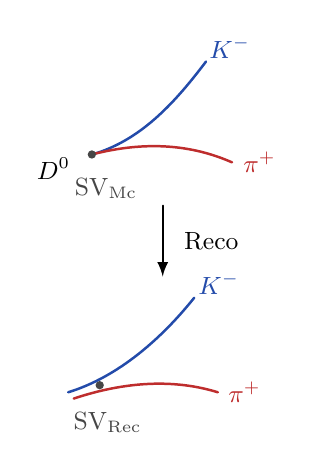
\begin{tikzpicture}[
    line cap=round,
    line join=round,
    every node/.style={font=\small}
]

\definecolor{kblue}{RGB}{35,75,170}
\definecolor{pired}{RGB}{190,45,45}
\definecolor{vtxgray}{RGB}{70,70,70}

% -----------------------------
% Top: generated topology
% -----------------------------
\coordinate (svmc) at (0,0);

\node[anchor=east] at (-0.15,-0.18) {$D^{0}$};

\draw[kblue, line width=0.9pt]
(svmc)
.. controls (0.65,0.18) and (1.10,0.72) ..
(1.45,1.18);

\draw[pired, line width=0.9pt]
(svmc)
.. controls (0.70,0.18) and (1.28,0.12) ..
(1.78,-0.10);

\fill[vtxgray] (svmc) circle (1.5pt);

\node[kblue, anchor=south west] at (1.37,1.10) {$K^{-}$};
\node[pired, anchor=west] at (1.80,-0.10) {$\pi^{+}$};

\node[vtxgray, anchor=north] at (0.18,-0.18)
{$\mathrm{SV}_{\mathrm{Mc}}$};

% -----------------------------
% Vertical reconstruction arrow
% -----------------------------
\draw[-latex, line width=0.8pt]
(0.90,-0.65) -- (0.90,-1.55)
node[midway,right=4pt] {Reco};

% -----------------------------
% Bottom: reconstructed topology
% -----------------------------
\begin{scope}[shift={(-3.85,-3.10)}]

\coordinate (svrec) at (3.85,0.18);

\draw[kblue, line width=0.9pt]
(3.55,0.08)
.. controls (4.20,0.28) and (4.75,0.78) ..
(5.15,1.28);

\draw[pired, line width=0.9pt]
(3.62,0.00)
.. controls (4.28,0.22) and (4.90,0.25) ..
(5.45,0.08);

\fill[vtxgray]
([xshift=1mm,yshift=-0.1mm]svrec) circle (1.5pt);

\node[kblue, anchor=south west] at (5.08,1.20) {$K^{-}$};
\node[pired, anchor=west] at (5.46,0.08) {$\pi^{+}$};

\node[vtxgray, anchor=north] at (4.05,-0.05)
{$\mathrm{SV}_{\mathrm{Rec}}$};

\end{scope}

\end{tikzpicture}

\end{document}
